\documentclass{article}
 
\usepackage[spanish]{babel}
\usepackage{listings}
\usepackage{epsfig} 
\usepackage{float}
 \usepackage{hyperref}
 \usepackage{color}
\usepackage{graphicx} % figuras
\usepackage{subfigure} % subfiguras
\usepackage[dvipsnames]{xcolor}
\usepackage{fancyvrb}
%\usepackage{multicol}
%\usepackage{url}
%\renewcommand{\UrlFont}{\small}
\setlength{\parskip}{0.25 cm}
\setlength{\parindent}{0pt}

                                                     %%%----------------------------------------------                 Datos personales             -----------------------------------------------------------
\title{Caracterización estructural de instancias.}
\author{4166}
%\institute{PISIS UANL}
%\email{hhector.garcialpz@uanl.edu.mx}
\date{\today}

\begin{document}
\maketitle
                                                           %%%--------------------------------------------                 Introduccion              -----------------------------------------------------
\section*{Introducción}
En un grafo formado por aristas y nodos, donde cada arista tiene un valor que se interpreta como la capacidad, algo de interés es, dado dos nodos identificados como \textbf{fuente} y \textbf{sumidero}, es saber cual es el valor del flujo máximo que puede transportar desde el fuente al sumidero. Otros aspectos importantes es ver como las caracteristicas del nodo fuente y el nodo sumidero afectan al valor del flujo máximo en el mismo grafo.

En este documento se habla acerca de las caracteristicas que presentan los nodos en un grafo y de que manera afectan estos en el valor del flujo máximo mediante un algoritmo de \texttt{Networkx}.

\section*{Especificaciones técnicas}
La computadora en la que se corrió los algoritmos es una Macbook Pro, cuyo procesador es un Intel Core i5 de 2.3 GHz. Tiene una memoria RAM de 8 GB 2133 MHz.

                                                          %%%--------------------------------------------                 Listings              -----------------------------------------------------
\definecolor{mygreen}{rgb}{0,0.6,0}
\definecolor{mygray}{rgb}{0.5,0.5,0.5}
\definecolor{mymauve}{rgb}{0.58,0,0.82}
\lstset{ 
  backgroundcolor=\color{white},   % choose the background color; you must add \usepackage{color} or \usepackage{xcolor}; should come as last argument
  basicstyle=\footnotesize,        % the size of the fonts that are used for the code
  breakatwhitespace=false,         % sets if automatic breaks should only happen at whitespace
  breaklines=true,                 % sets automatic line breaking
  captionpos=b,                    % sets the caption-position to bottom
  commentstyle=\color{mygreen},    % comment style
  deletekeywords={...},            % if you want to delete keywords from the given language
  escapeinside={\%*}{*)},          % if you want to add LaTeX within your code
  extendedchars=true,              % lets you use non-ASCII characters; for 8-bits encodings only, does not work with UTF-8
  firstnumber=1,                % start line enumeration with line 1000
  frame=single,	                   % adds a frame around the code
  keepspaces=true,                 % keeps spaces in text, useful for keeping indentation of code (possibly needs columns=flexible)
  keywordstyle=\color{blue},       % keyword style
  language=Octave,                 % the language of the code
  morekeywords={*,...},            % if you want to add more keywords to the set
  numbers=left,                    % where to put the line-numbers; possible values are (none, left, right)
  numbersep=5pt,                   % how far the line-numbers are from the code
  numberstyle=\tiny\color{mygray}, % the style that is used for the line-numbers
  rulecolor=\color{black},         % if not set, the frame-color may be changed on line-breaks within not-black text (e.g. comments (green here))
  showspaces=false,                % show spaces everywhere adding particular underscores; it overrides 'showstringspaces'
  showstringspaces=false,          % underline spaces within strings only
  showtabs=false,                  % show tabs within strings adding particular underscores
  stepnumber=1,                    % the step between two line-numbers. If it's 1, each line will be numbered
  stringstyle=\color{mymauve},     % string literal style
  tabsize=2,	                   % sets default tabsize to 2 spaces
  title=\lstname                   % show the filename of files included with \lstinputlisting; also try caption instead of title
}
                                                            %%%--------------------------------------------                 Generadores             -----------------------------------------------------
\section{Generador}

\subsection*{\texttt{watts\_strogatz\_graph()}}
Este generador de grafos toma como parámetros la cantidad de nodos deseados, el numero de nodos vecinos con los que se puede conectar y la probabilidad de conexión desde ese nodo con los nodos que puede conectar.

Usualmente, este tipo de grafos, se usa para hacer las redes de mundo pequeño estas redes hacen referencia a que por mas alejado que esté un nodo del otro, todos los nodos son accesibles desde otro nodo.

En las figuras \ref{muestra0}, \ref{muestra1}, \ref{muestra2}, \ref{muestra3}, \ref{muestra4} se muestran grafos que son hechos con este generador.

\begin{figure}
\centering
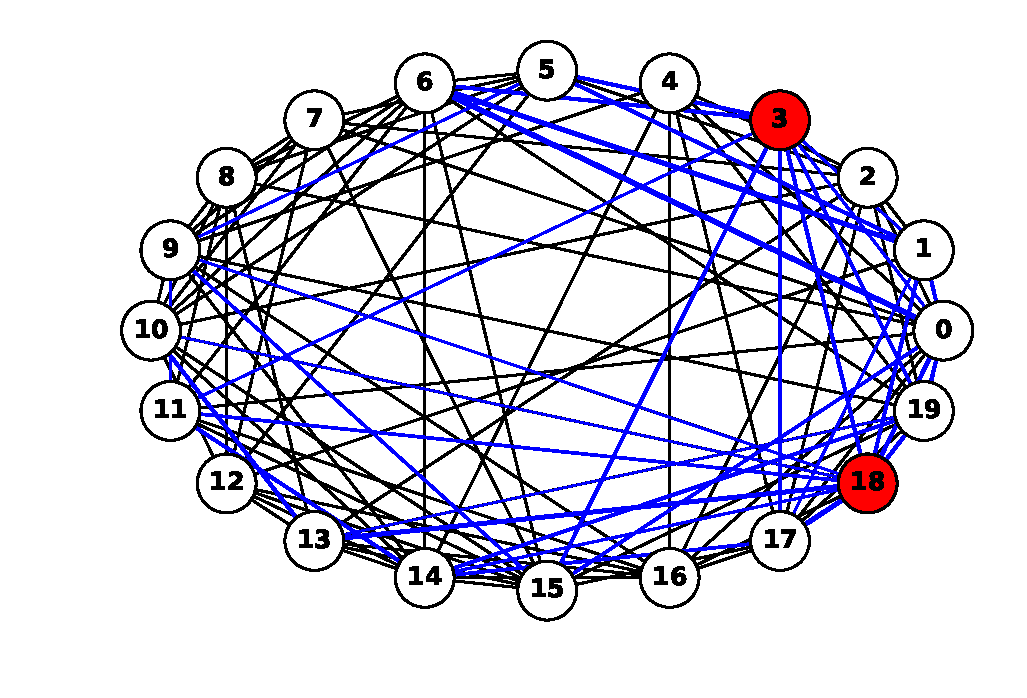
\includegraphics [width=130mm] {muestra0.eps}
\caption{Grafo con rutas de flujo máimo.}
\label{muestra0}
\end{figure}

\begin{figure}
\centering
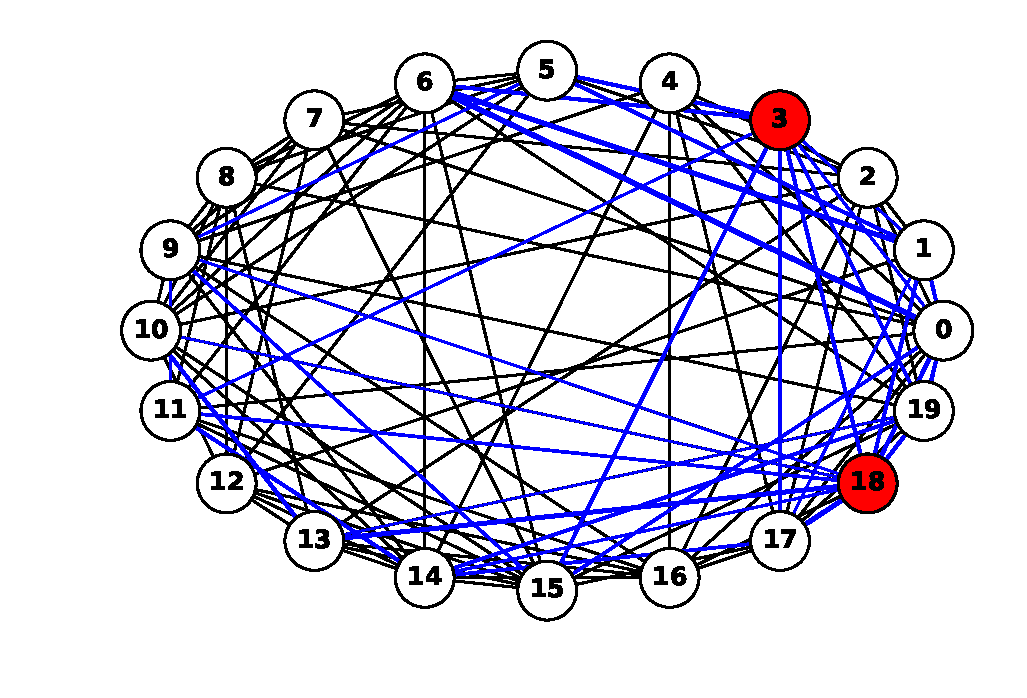
\includegraphics [width=130mm] {muestra0.eps}
\caption{Grafo con rutas de flujo máimo.}
\label{muestra1}
\end{figure}

\begin{figure}
\centering
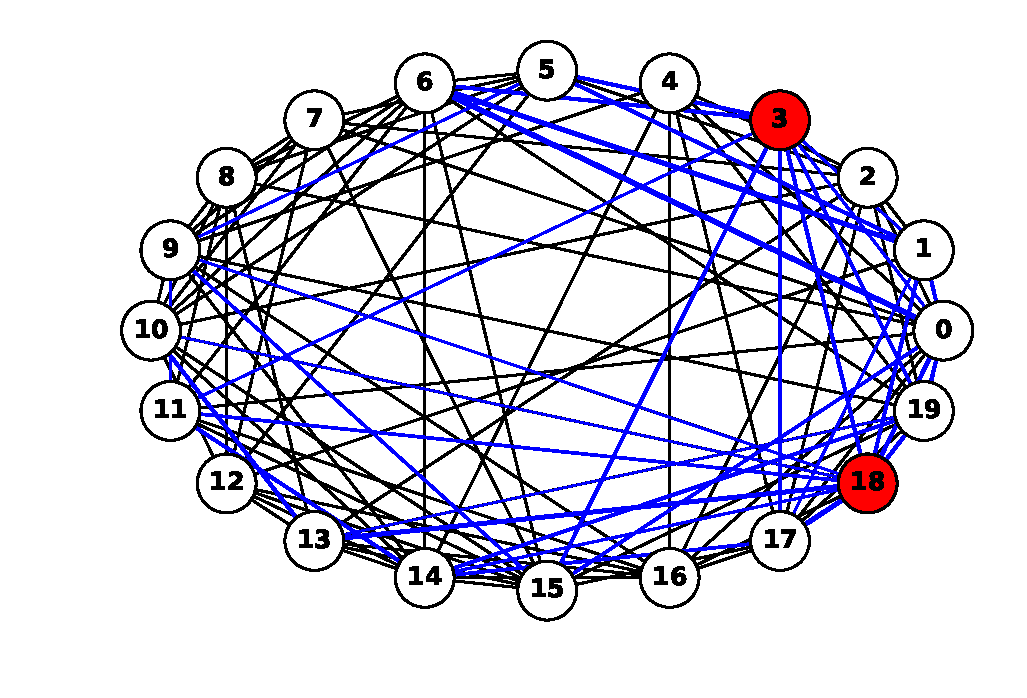
\includegraphics [width=130mm] {muestra0.eps}
\caption{Grafo con rutas de flujo máimo.}
\label{muestra2}
\end{figure}

\begin{figure}
\centering
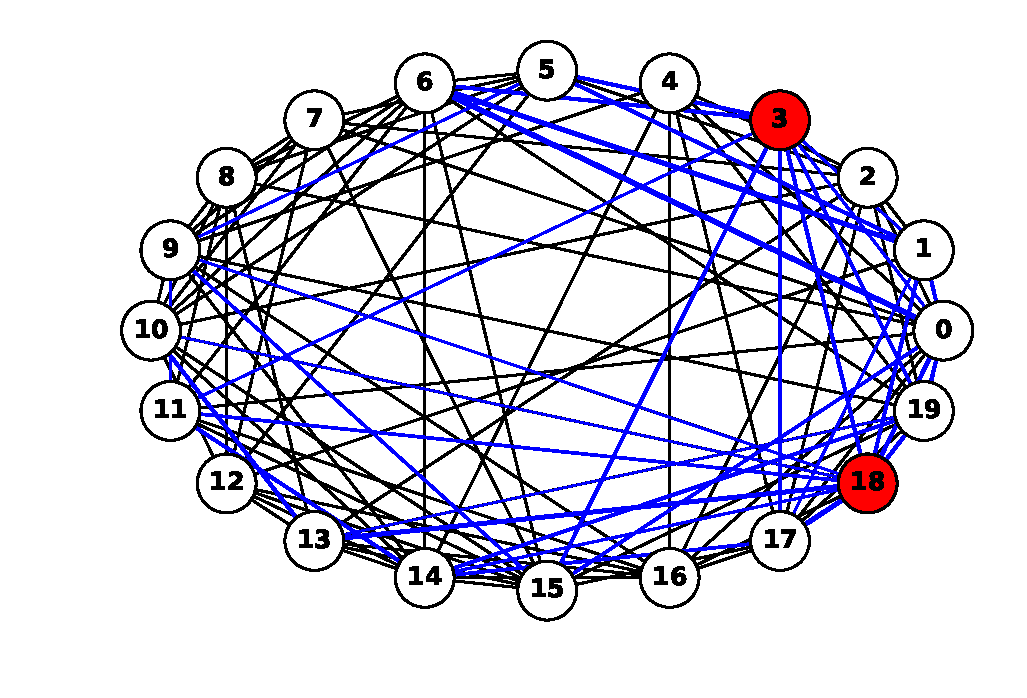
\includegraphics [width=130mm] {muestra0.eps}
\caption{Grafo con rutas de flujo máimo.}
\label{muestra3}
\end{figure}

\begin{figure}
\centering
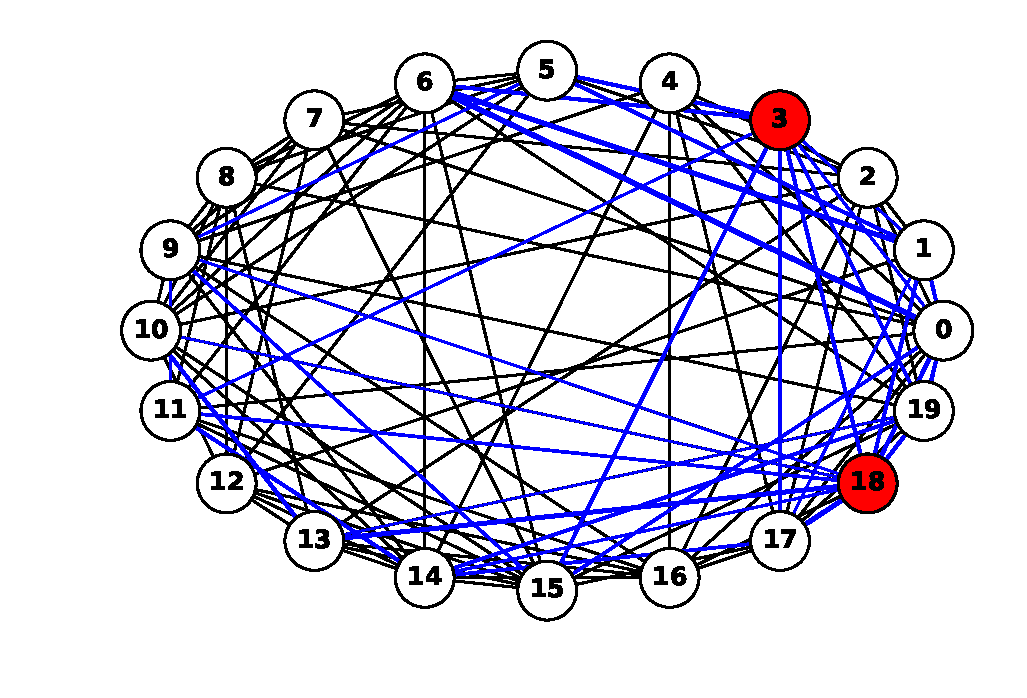
\includegraphics [width=130mm] {muestra0.eps}
\caption{Grafo con rutas de flujo máimo.}
\label{muestra4}
\end{figure}

                                                                %%%--------------------------------------------                 Algoritmo              -----------------------------------------------------
\section*{Algoritmos}
En esta sección se habla de los algoritmos que se usaron junto con una breve descripción.

\subsection*{Algoritmo de flujo máximo}
El algoritmo implementado para encontrar el flujo máximo es \texttt{maximum\_flow()} el cual toma como parámetros un grafo el cual debe tener como atributo la capacidad de cada arista, junto con el par de nodos fuente y sumidero. Al encontrar el flujo máximo devuelve el valor de este, asi como el flujo que pasa por cada arista para obtener ese valor del flujo máximo.

\subsection*{\texttt{degree\_centrality()}}


\subsection*{\texttt{clustering()}}
Este algoritmo que recibe como parámetro un grafo que puede ser con pesos en sus aristas o sin pesos; el caso que se tiene aristas con pesos, devuelve el promedio geométrico de los pesos del subgrafo.

\subsection*{\texttt{closeness\_centrality()}}
Mediante este algoritmo se obtiene una medida de centralidad de la red, es decir, para cada nodo se calcula que tan central es; entre más al centro esté el nodo está mas cerca de todos los demás nodos. 

\subsection*{\texttt{load\_centrality()}}
Una vez que se obtienen todas las rutas mas cortas, el dato que ofrece este algoritmo es la fracción de todas las rutas mas cortas que pasan a través de ese nodo.

\subsection*{\texttt{eccentricity()}}
La información que aporta este algoritmo es para determinar que tan cerca o tan lejos está un nodo con respecto a los demás.

\subsection*{\texttt{pagerank()}}
Este algoritmo calcula una clasificación de los nodos en el gráfico de acuerdo a las características de los nodos con quien esta conectado.

                                                                    %%%--------------------------------------------                 Metodología              -----------------------------------------------------
\section{Metodología}
El interés de este estudio es determinar qué características de los nodos influyen en un mayor valor de flujo máximo. Lo que se hace es generar un grafo de diferentes tamaños, desde veinte nodos hasta sesenta nodos con incrementos de diez nodos, una vez que el grafo ya tiene capacidad se eligen los pares de nodos fuente y sumidero, se calcula el valor del flujo máximo y se guarda las características que tienen éstos nodos.

\newpage
La implementación en python se lleva a cabo con el código siguiente.
\lstinputlisting[language=Python, firstline=65, lastline=105]{caracterizacion.py}


                                                                       %%%--------------------------------------------                 Resultados              -----------------------------------------------------
\section{Resultados}
Se elaboró unos diagramas de caja para ver el comportamiento de las características de los nodos fuente y sumidero \ref{tiempo}, \ref{clsnsfuente}, \ref{clsnssumidero}, \ref{clstrfuente}, \ref{clstrsumidero}, \ref{loadfuente}, \ref{loadsumidero}, \ref{pagefuente}, \ref{pagesumidero}. Los valores del eje de las abscisas representan el orden de los grafos.

\begin{figure}
\centering
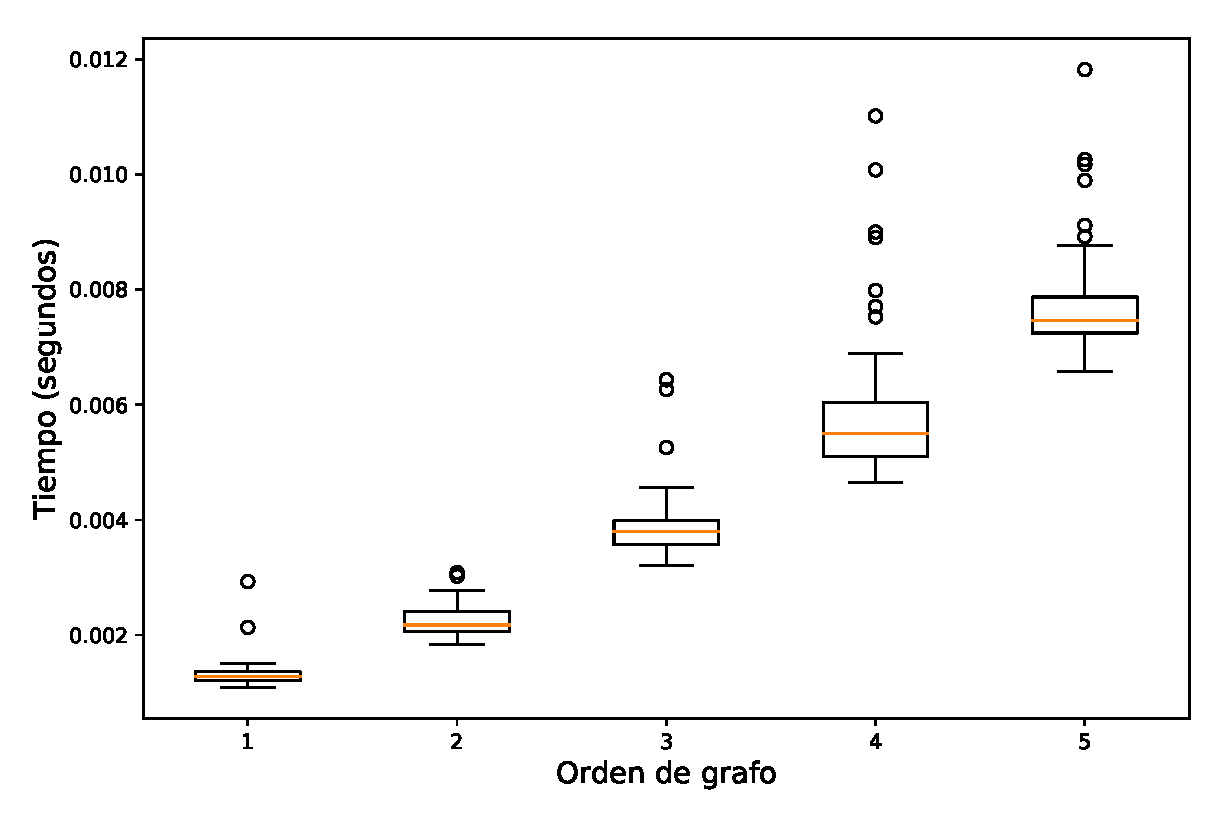
\includegraphics [width=90mm] {boxtiempo.eps}
\caption{Diagrama de caja de tiempo.}
\label{tiempo}
\end{figure}

\begin{figure}
\centering
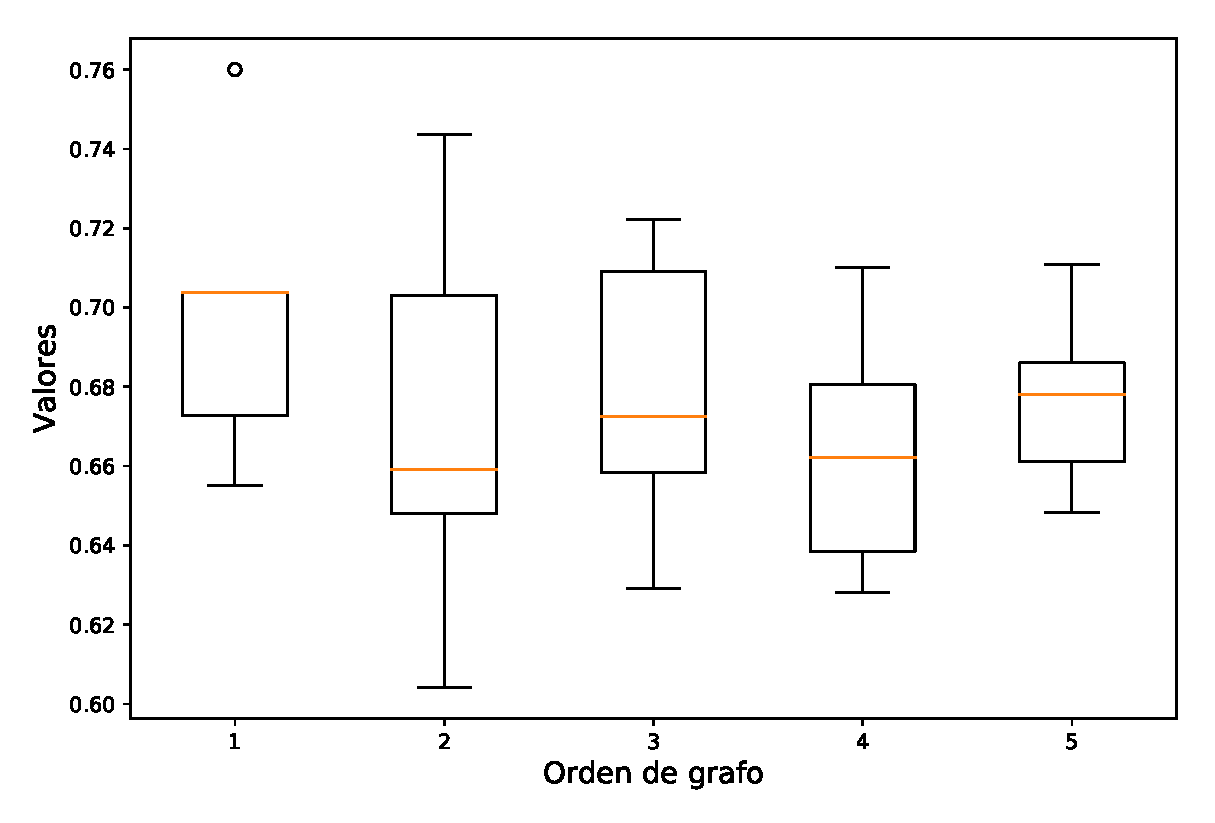
\includegraphics [width=90mm] {box_clsnsfuente.eps}
\caption{Diagrama de caja de centralidad de nodos fuentes.}
\label{clsnsfuente}
\end{figure}

\begin{figure}
\centering
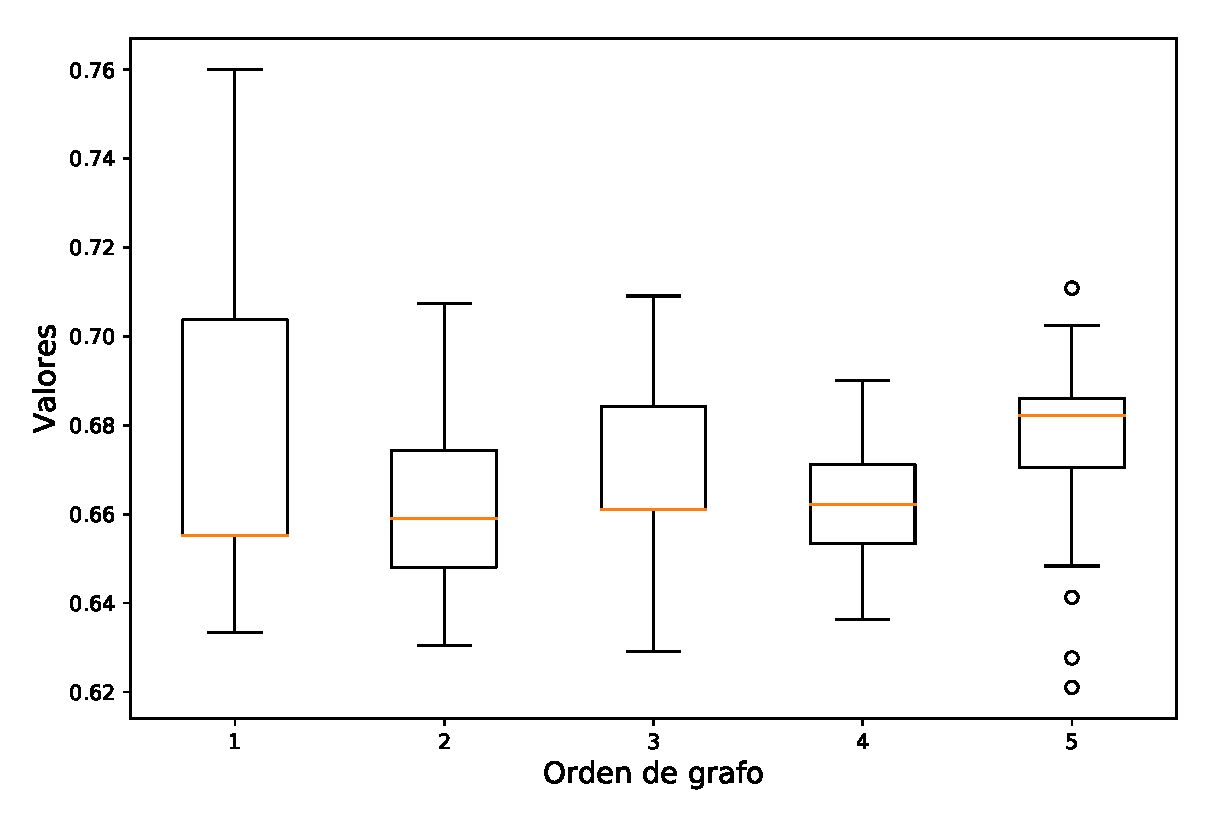
\includegraphics [width=90mm] {box_clsnssumidero.eps}
\caption{Diagrama de caja de centralidad de nodos sumidero.}
\label{clsnssumidero}
\end{figure}

\begin{figure}
\centering
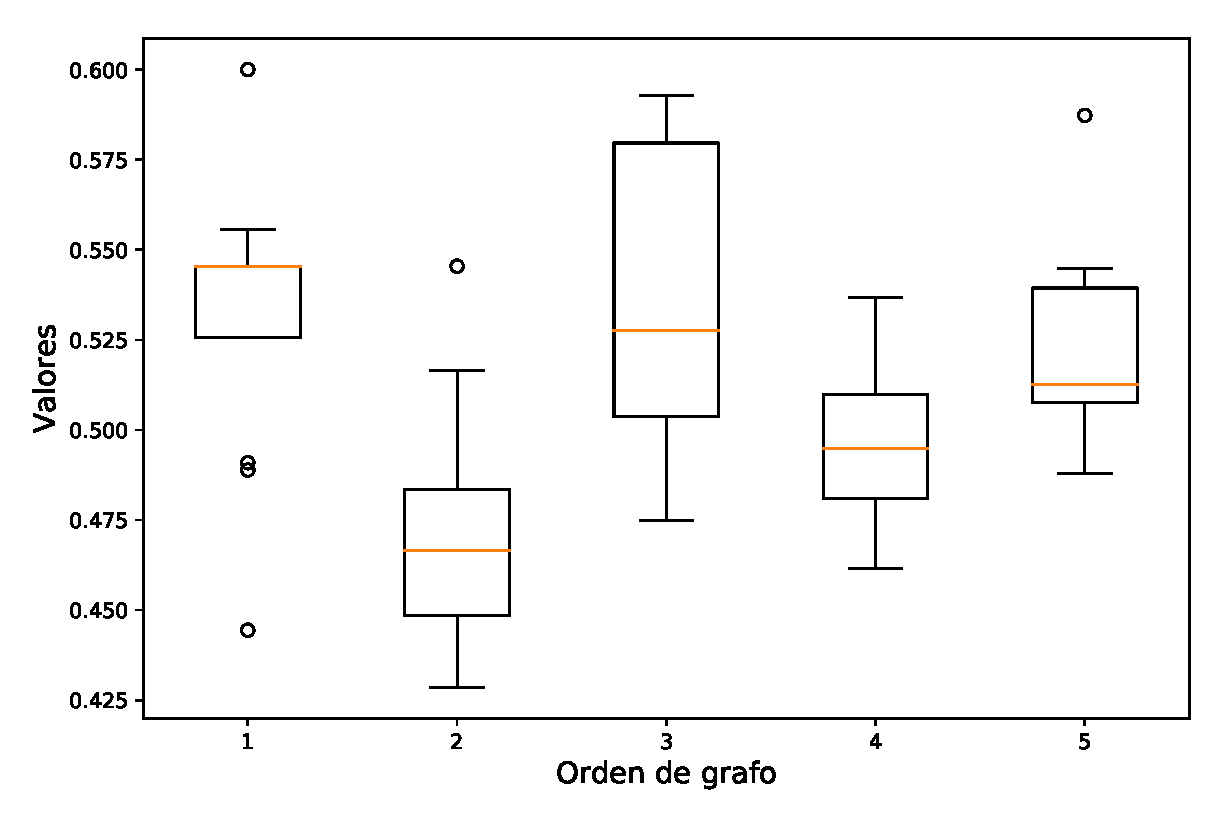
\includegraphics [width=90mm] {box_clstrfuente.eps}
\caption{Diagrama de caja de clustering de nodos fuentes.}
\label{clstrfuente}
\end{figure}

\begin{figure}
\centering
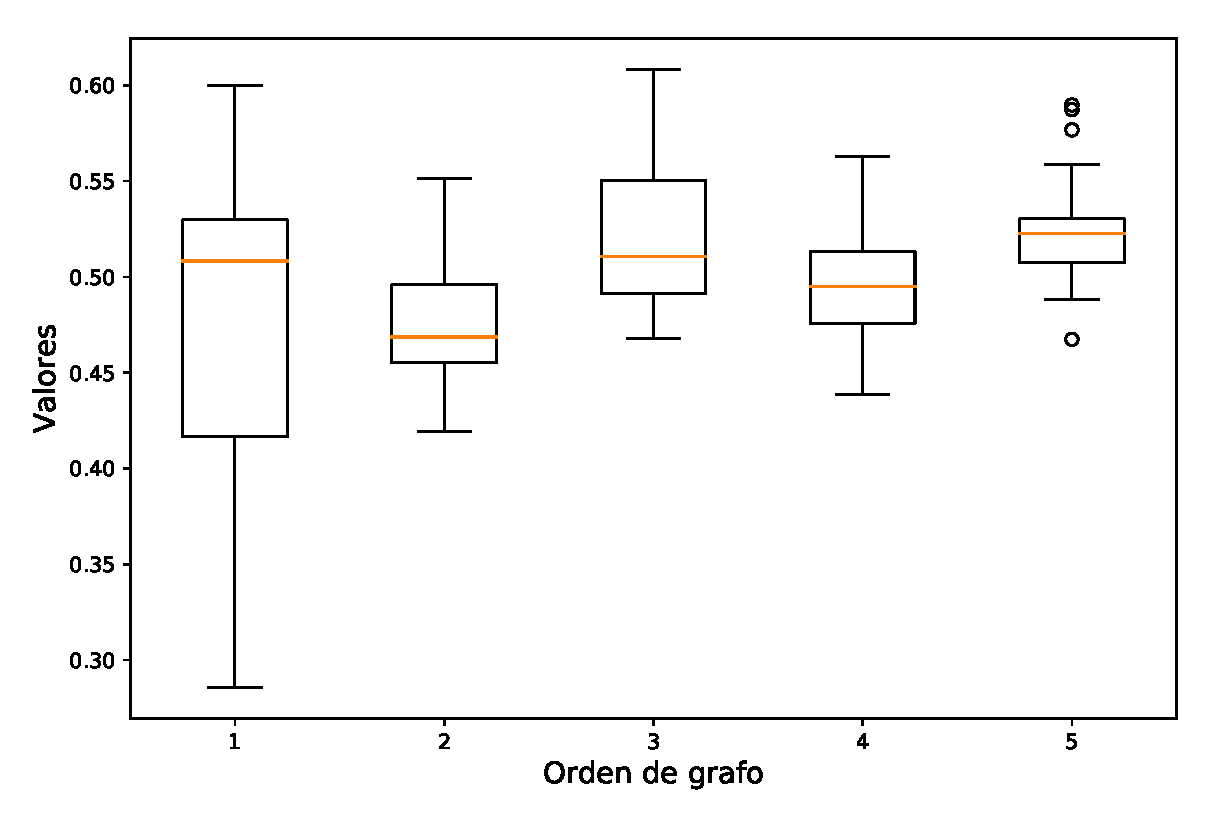
\includegraphics [width=90mm] {box_clstrsumidero.eps}
\caption{Diagrama de caja de clustering de nodos sumidero.}
\label{clstrsumidero}
\end{figure}

\begin{figure}
\centering
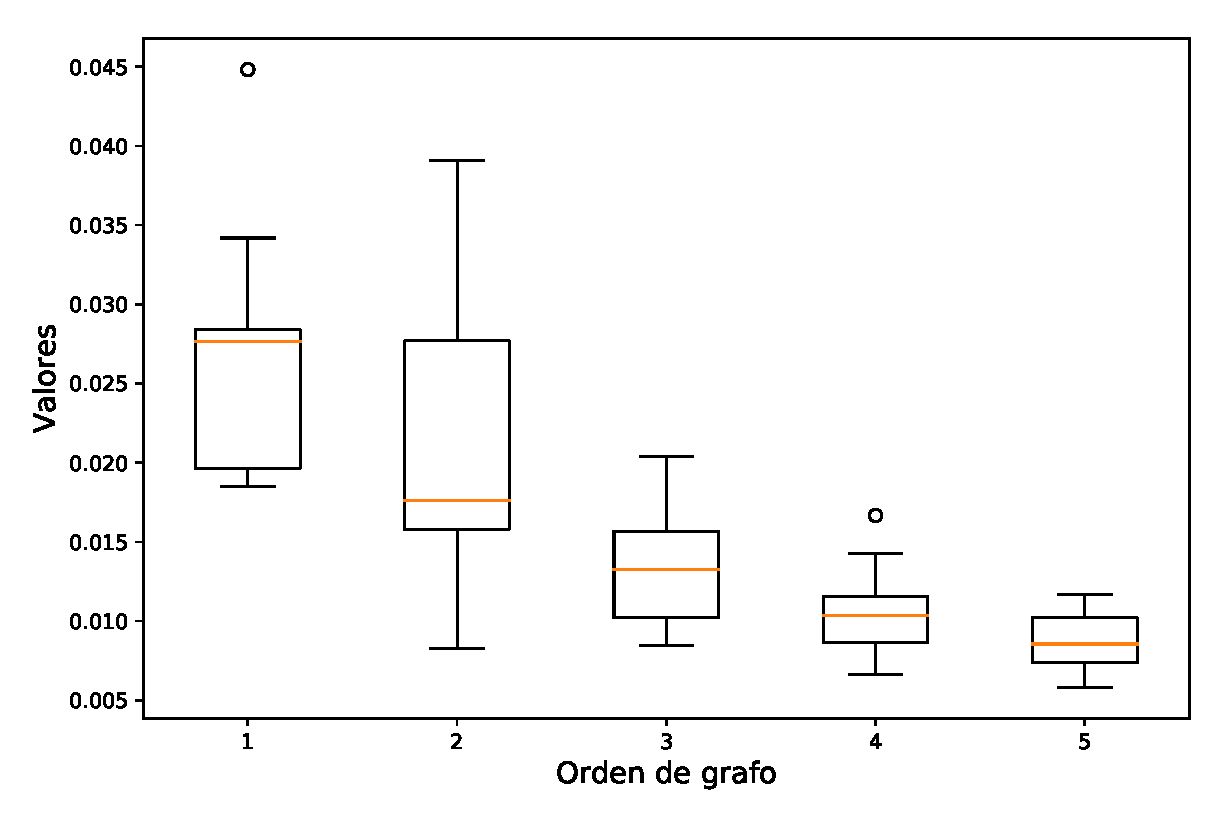
\includegraphics [width=90mm] {box_loadfuente.eps}
\caption{Diagrama de caja de load centrality de nodos fuentes.}
\label{loadfuente}
\end{figure}

\begin{figure}
\centering
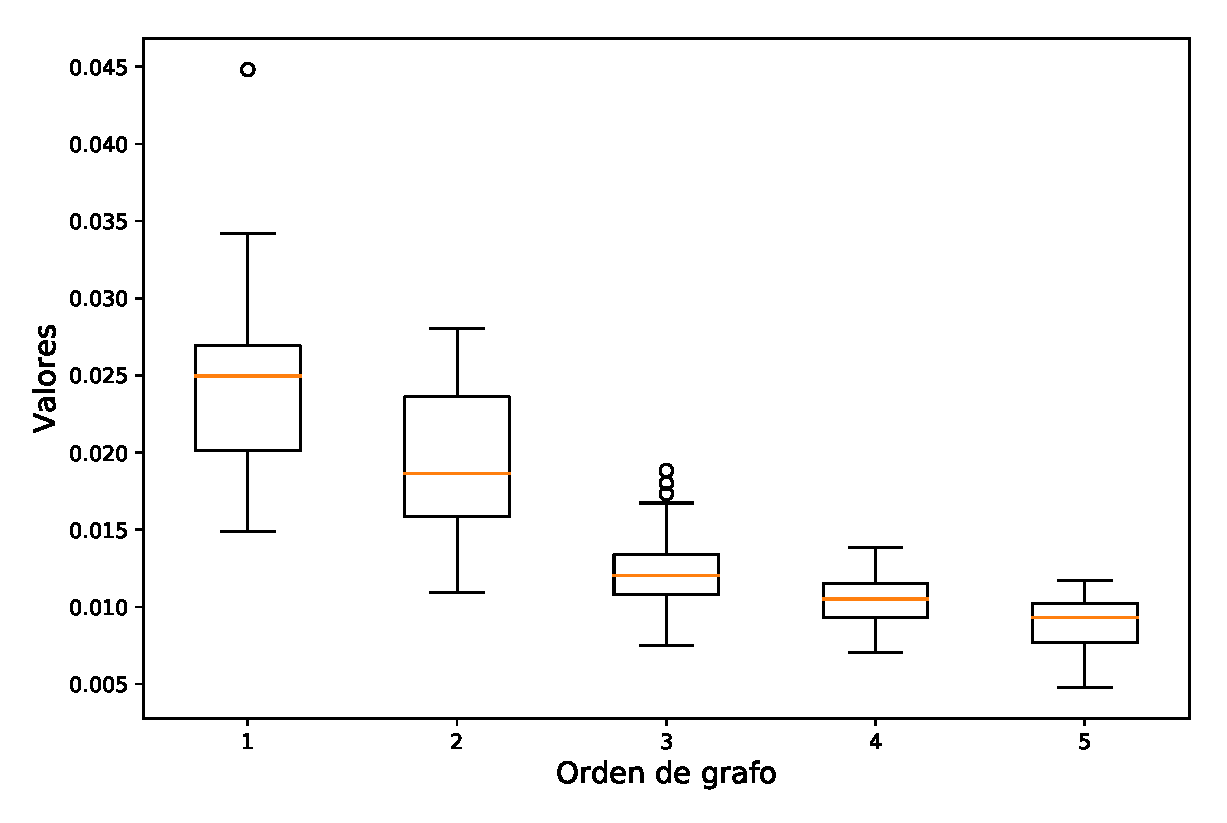
\includegraphics [width=81mm] {box_loadsumidero.eps}
\caption{Diagrama de caja de load centrality de nodos sumidero.}
\label{loadsumidero}
\end{figure}

\begin{figure}
\centering
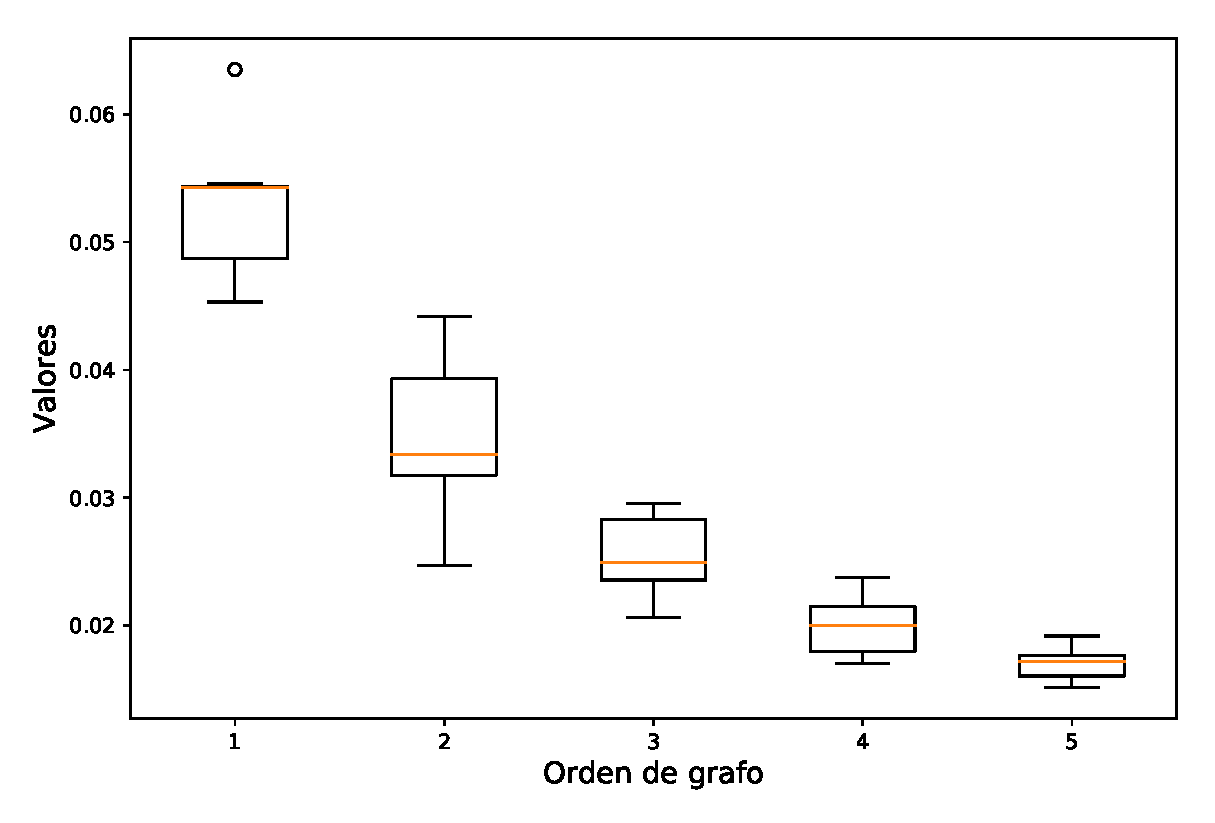
\includegraphics [width=90mm] {box_pagefuente.eps}
\caption{Diagrama de caja de pagerank de nodos fuentes.}
\label{pagefuente}
\end{figure}

\begin{figure}
\centering
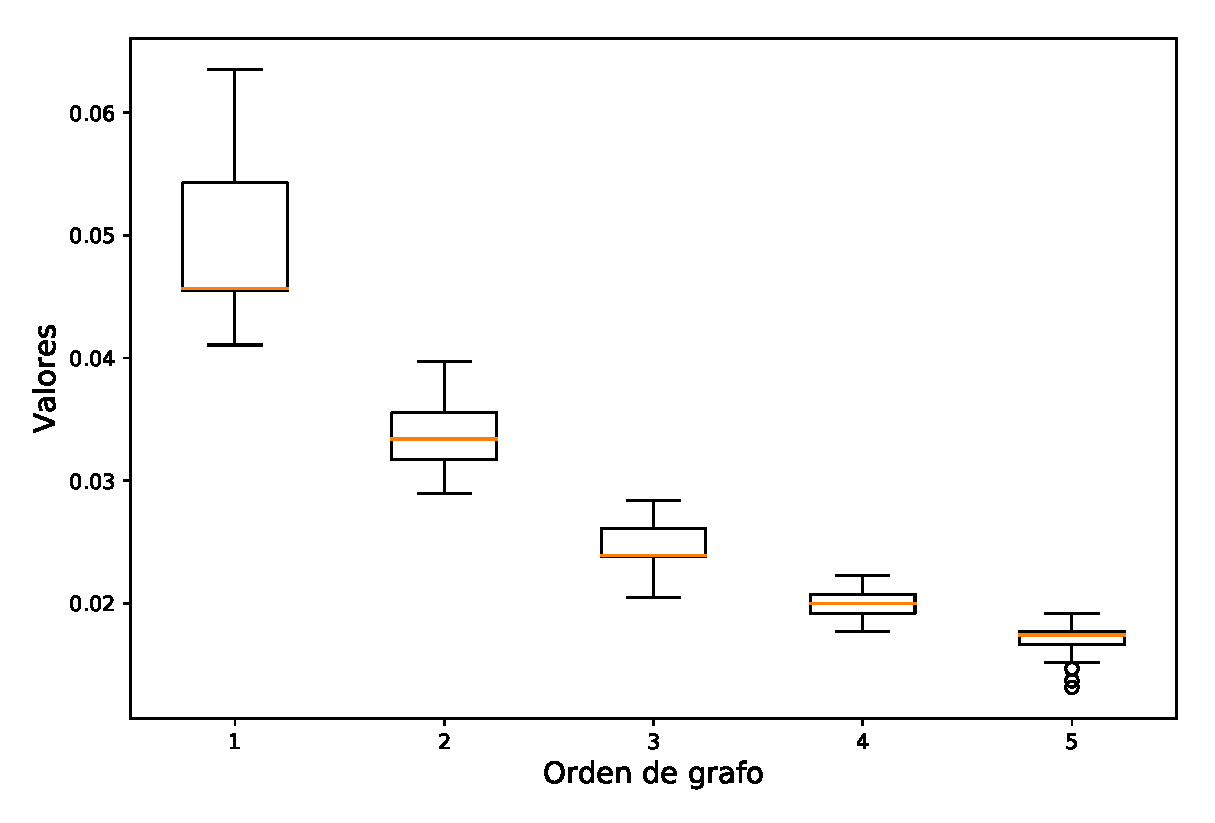
\includegraphics [width=90mm] {box_pagesumidero.eps}
\caption{Diagrama de caja de load pagerank de nodos sumidero.}
\label{pagesumidero}
\end{figure}

Con esa información se hace una matriz de correlación \ref{correlacion} donde el cero es el valor del flujo máximo, el uno es el valor del tiempo, la fila cinco es el valor de load centrality del nodo fuente, el siete representa el pagerank del nodo fuente, las filas once y trece es el valor de load centrality y pagerank del nodo sumidero respectivamente.

Las filas y columnas en negro, es debido a que representan la excentricidad y su valor permanece constante para todos los grafos.

\begin{figure}
\centering
\includegraphics [width=100mm] {Correlaciones.eps}
\caption{Correlaciones de las características de los nodos fuente y sumidero.}
\label{correlacion}
\end{figure}

Lo que nos muestra \ref{correlacion} es que el valor de load centrality y el pagerank, tanto del nodo fuente como del sumidero afectan inversamente al valor del flujo máximo.

Luego, se hizo un ANOVA para identificar si las medias de los conjuntos eran iguales o hay diferencias significativas en ellas. Se obtuvo los resultados que se muestra en la tabla llamada \texttt{ANOVA.txt} en el cual los valores de la tercer columna que son mayores a 0.1, sus medias son iguales y los valores menores 0.1 se rechaza la hipótesis de que las medias sean iguales.

% redefine \VerbatimInput
\RecustomVerbatimCommand{\VerbatimInput}{VerbatimInput}
{fontsize=\footnotesize,
 %
 frame=lines, % top and bottom rule only
 framesep=2em,% separation between frame and text
 rulecolor=\color{Gray},
 %
 label=\fbox{\color{Black}ANOVA.txt},
 labelposition=topline,
 %
 commandchars=\|\(\), % escape character and argument delimiters for
                      % commands within the verbatim
 commentchar=*        % comment character
}

\VerbatimInput{Anova1.txt}




\bibliographystyle{IEEEtran}
\bibliography{Bibliog}
\nocite{*}
\end{document}
